\subsection{Quinto sprint}

\begin{minipage}{\textwidth}
  Di seguito è riportata la distribuzione delle ore per ciascun membro del team, accumulate in totali per persona e per ruolo:
  \begin{table}[H]
    \begin{tabularx}{\textwidth}{|c|*{6}{>{\centering}X|}c|}
      \hline
      \multicolumn{8}{|c|}{\textbf{Consuntivo orario}} \\
      \hline
      \textbf{Membro del team} & \textbf{Re} & \textbf{Am} & \textbf{An} & \textbf{Pt} & \textbf{Pr} & \textbf{Ve} & \textbf{Totale per persona} \\
      \hline
      Cavalli Riccardo & 0 & 1 & 2 & 0 & 2 & 1 & 6 \\ \hline
      Pianon Raul & 0 & 0 & 0 & 0 & 5 & 0 & 5 \\ \hline
      Dall’Amico Martina & 3 & 0 & 0 & 0 & 0 & 3 & 6 \\ \hline
      Cristo Marco & 1 & 0 & 0 & 0 & 3 & 2 & 6 \\ \hline
      Lewental Sebastiano & 0 & 0 & 0 & 0 & 3 & 2 & 5 \\ \hline
      Zecchinato Mattia & 0 & 1 & 0 & 0 & 4 & 0 & 5 \\ \hline
      Stocco Tommaso & 0 & 0 & 0 & 0 & 3 & 0 & 3 \\ \hline
      \textbf{Totale ore per ruolo} & 4 & 2 & 2 & 0 & 20 & 8 & \textbf{36} \\
      \hline
    \end{tabularx}
    \caption{Sprint 5 - Consuntivo orario}
  \end{table}
  \end{minipage}
  
  \begin{figure}[H]
    \centering
    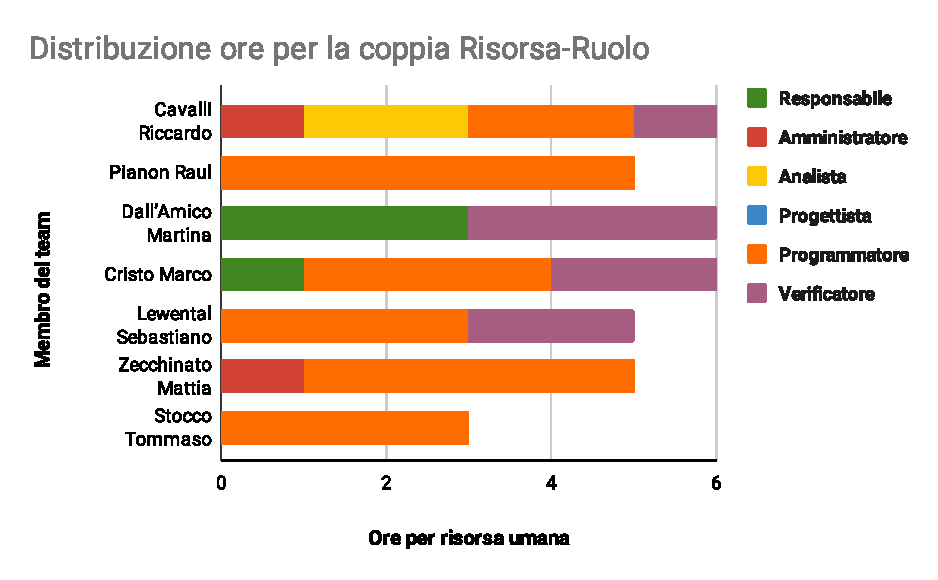
\includegraphics[width=0.90\textwidth]{assets/Consuntivo/Sprint-5/distribuzione_ore_risorsa_ruolo.pdf}
    \caption{Sprint 5 - Istogramma della distribuzione oraria per la coppia risorsa-ruolo}
  \end{figure}
  
  \begin{figure}[H]
    \centering
    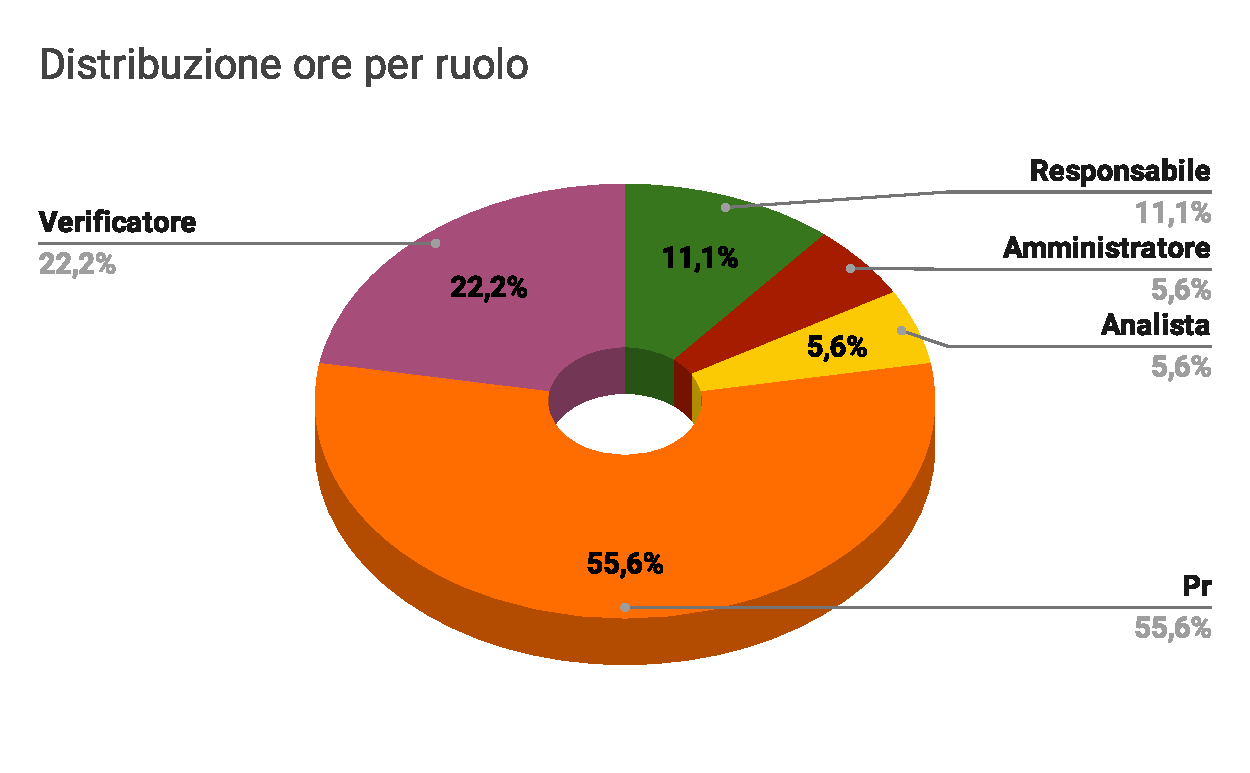
\includegraphics[width=0.90\textwidth]{assets/Consuntivo/Sprint-5/distribuzione_ore_ruolo.pdf}
    \caption{Sprint 5 - Areogramma della distribuzione oraria per ruolo}
  \end{figure}
  
  \begin{minipage}{\textwidth}
  Di seguito è riportato il consuntivo economico del quinto \glossario{sprint}:
  \begin{table}[H]
  \begin{adjustwidth}{-0.5cm}{-0.5cm}
    \centering
    \begin{tabular}{|P{2.9cm}|P{2.3cm}|P{2.5cm}|P{2.3cm}|>{\arraybackslash}P{2.5cm}|}
      \hline
      \multicolumn{5}{|c|}{\textbf{Consuntivo economico}} \\
      \hline
      \textbf{Ruolo} & \textbf{Ore per ruolo} & \textbf{Delta ore preventivo - consuntivo} & \textbf{Costo (in \texteuro)} & \textbf{Delta costo preventivo - consuntivo (in \texteuro)} \\
      \hline
      Responsabile & 4 & 0 & 120,00 & 0,00 \\ \hline
      Amministratore & 2 & 1 & 40,00 & 20,00 \\ \hline
      Analista & 2 & 1 & 50,00  & 25,00 \\ \hline
      Progettista &  0 & 0 & 0,00 & 0,00 \\ \hline
      Programmatore & 20 & 2 & 300,00 & 30,00 \\ \hline
      Verificatore & 8 & -3 & 120,00 & -45,00 \\ \hline
      \textbf{Totale} & \textbf{36} & 1 & \textbf{630,00} & 30,00 \\ \hline
    \textbf{Restante} & 410 & / & 8.115,00 & / \\ \hline
      \textbf{Sprint pregressi} & 200 & / & 4.275,00 & / \\ \hline
    \end{tabular}
    \caption{Sprint 5 - Consuntivo economico}
  \end{adjustwidth}
  \end{table}
  \end{minipage}
  
  \begin{figure}[H]
    \centering
    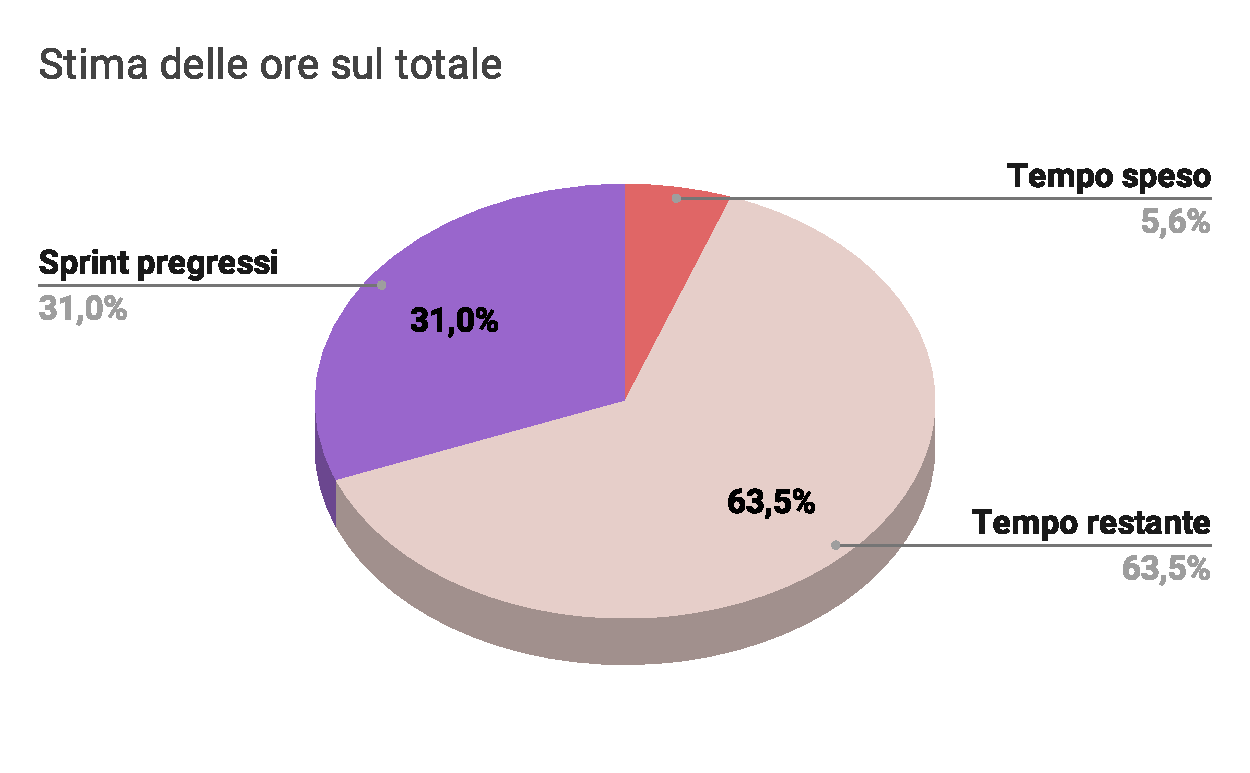
\includegraphics[width=0.90\textwidth]{assets/Consuntivo/Sprint-5/copertura_oraria.pdf}
    \caption{Sprint 5 - Areogramma del tempo speso (in ore) rispetto al totale}
  \end{figure}
  
  \begin{figure}[H]
    \centering
    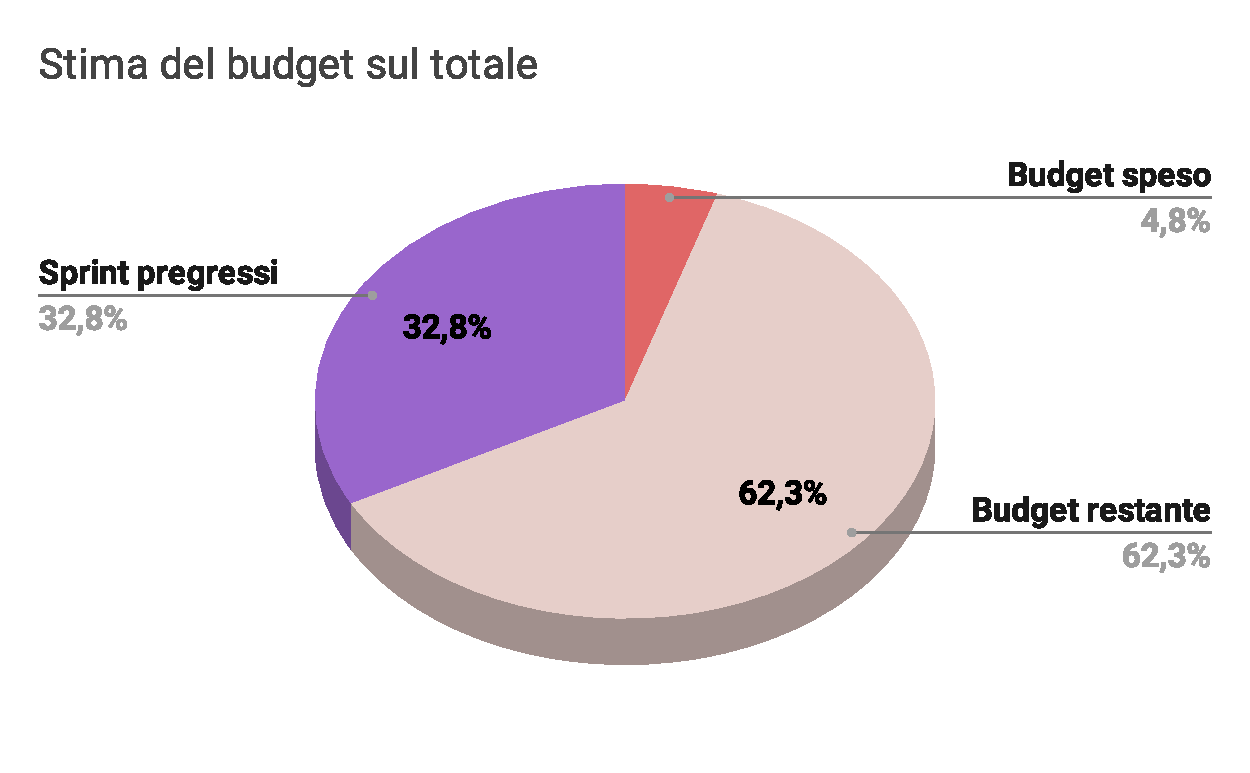
\includegraphics[width=0.90\textwidth]{assets/Consuntivo/Sprint-5/budget_speso.pdf}
    \caption{Sprint 5 - Areogramma del budget speso rispetto al totale}
  \end{figure}
  
  \begin{minipage}{\textwidth}
    Di seguito sono riportate le ore rimanenti per la coppia risorsa-ruolo:
    \begin{table}[H]
      \begin{tabularx}{\textwidth}{|c|*{6}{>{\centering}X|}c|}
        \hline
        \multicolumn{8}{|c|}{\textbf{Ore rimanenti per la coppia risorsa-ruolo}} \\
        \hline
        \textbf{Membro del team} & \textbf{Re} & \textbf{Am} & \textbf{An} & \textbf{Pt} & \textbf{Pr} & \textbf{Ve} & \textbf{Totale per persona} \\
        \hline
        Cavalli Riccardo & 0 & 1 & 7 & 14 & 16 & 15 & 53 \\ \hline
        Pianon Raul & 2 & 10 & 2 & 20 & 10 & 12 & 56 \\ \hline
        Dall’Amico Martina & 6 & 2 & 1 & 14 & 22 & 13 & 58 \\ \hline
        Cristo Marco & 2 & 10 & 2 & 17 & 10 & 15 & 56 \\ \hline
        Lewental Sebastiano & 9 & 4 & 2 & 11 & 18 & 15 & 59 \\ \hline
        Zecchinato Mattia & 9 & 8 & 3 & 11 & 16 & 15 & 62 \\ \hline
        Stocco Tommaso & 5 & 4 & 3 & 20 & 13 & 19 & 64 \\ \hline
        \textbf{Totale ore per ruolo} & 33 & 40 & 20 & 107 & 106 & 104 & \textbf{410} \\ 
        \hline
      \end{tabularx}
      \caption{Sprint 5 - Ore rimanenti per la coppia risorsa-ruolo}
    \end{table}
  \end{minipage}

\subsubsection{Revisione delle attività}

Nell'arco del quinto \glossario{sprint}, il team ha svolto le seguenti attività:
\begin{itemize}
  \item Stesura del consuntivo dello sprint 4;
  \item Completamento della formalizzazione della dashboard \glossario{Google Sheets} nelle \NdP;
  \item Completamento della spiegazione delle funzionalità e specifiche dei vari documenti nelle \NdP;
  \item Stesura del verbale interno del 03/06;
  \item Stesura del preventivo e della pianificazione dello sprint 5 nel \PdP;
  \item Ampliamento delle \AdR con grafici e aggiunta casi d’uso;
  \item Configurazione di Flask con Vue.js;
  \item Integrazione tra \glossario{back-end} e \glossario{front-end};
  \item Connessione al \glossario{database} con Flask;
  \item Implementazione delle funzionalità di Login e Logout con FastAPI nel \glossario{back-end};
  \item Gestione delle operazioni \glossario{CRUD} per il \glossario{dizionario dati} nel backend;
  \item Ultimi approfondimenti sul funzionamento di \glossario{txtai};
  \item Sviluppo del \glossario{front-end} per il ChatBOT;
  \item Progettazione e sviluppo dei casi d’uso nel \glossario{front-end};
  \item Modifica del \glossario{dizionario dati}, inclusa la descrizione delle tabelle e delle chiavi esterne;
  \item Aggiornamento del prompt generator dopo l'incontro con la \glossario{Proponente};
  \item Riorganizzazione del file di \glossario{log}.
  \item Test del dizionario dati in italiano;
  \item Aggiunta di test con modelli locali.
\end{itemize}

\subsubsection{Retrospettiva}

\par Di seguito sono riportati i risultati del questionario di valutazione dello \glossario{sprint}:
\begin{itemize}
  \item Organizzazione dello \glossario{sprint}\ - Valutazione: 8,2;
  \item Conduzione dei meeting interni - Valutazione: 8,2;
  \item Conduzione dei meeting esterni - Valutazione: 8,8;
  \item Impegno e partecipazione dei singoli membri - Valutazione: 7,5;
  \item La quasi totalità dei membri del team era a conoscenza delle proprie mansioni;
  \item La numerosità delle riunioni è risultata adeguata;
  \item Le riunioni sono state organizzate sempre con il giusto preavviso;
  \item Il rapporto ore spese/ore produttive ha avuto un miglioramento significativo e un bilanciamento equo tra i membri del gruppo;
  \item La produttività generale ha raggiunto una buona soglia;
  \item Alcuni membri del team hanno messo in luce la necessità di una frequanza maggiore di aggiornamento del \glossario{repository} di ChatSql.
\end{itemize}

\vspace{0.5\baselineskip}
\par A seguire le \textbf{analisi a posteriori} del quinto \glossario{sprint}:
\begin{itemize}
  \item Miglioramento dell'Efficienza: Il team ha riscontrato un miglioramento nel rapporto tra ore produttive e ore di orologio spese per portare a termine i task stabiliti. Questo è dovuto alla migliore organizzazione che, con l'aumentare degli sprint e dell'esperienza, sta maturando. Inoltre, il minor bisogno di imparare nuove tecnologie e l'applicazione delle conoscenze acquisite in precedenza hanno contribuito a questo miglioramento;
  \item Adozione delle Nuove Tecnologie: Il passaggio alle nuove tecnologie è stato repentino ma non complicato. Negli sprint precedenti, tutte le ipotesi sulle varie tecnologie erano state valutate e approfondite, inclusi Vue.js e Flask. Questo ha permesso al team di adattarsi rapidamente e di integrare efficacemente le nuove tecnologie nel progetto;
  \item Incontro con la Proponente: Durante lo sprint, è stato organizzato un incontro con la Proponente, durante il quale è stata mostrata una demo del progetto. I riscontri ricevuti sono stati positivi e costruttivi. Dall'incontro sono emersi nuovi casi d'uso e nuovi test da sviluppare, che assicureranno un miglioramento del prodotto finale;
  \item Aggiornamento del repository: un'area di miglioramento individuata riguarda l'aggiornamento del \glossario{repository} ChatSQL. Per mantenere il team allineato rispetto al lavoro dei programmatori, è necessario aggiornare l'ambiente condiviso con maggiore frequenza. Pertanto, si è stabilito di applicare con più costanza la pratica di \glossario{continuous integration}, invece di effettuare commit con minore frequenza e maggiore volume. Con questo approccio, il team ritiene di poter ottimizzare sia la verifica che lo sviluppo, riducendo il rischio di conflitti;
  \item Comprensione dei Casi d'Uso: Una difficoltà riscontrata è stata la comprensione del legame tra i casi d'uso. Questo aspetto è stato approfondito durante un incontro con il Professor Cardin, in cui è stato esaminato un caso d'uso specifico relativo alla generazione del prompt. L'incontro ha permesso di chiarire i ragionamenti e le motivazioni alla base della struttura attuale e ha fornito indicazioni sui miglioramenti da apportare nel prossimo sprint.
\end{itemize}

In conclusione, lo sprint 5 ha visto significativi progressi in termini di efficienza e adozione delle tecnologie, nonché preziosi feedback e direzioni per migliorare ulteriormente il progetto.


\subsubsection{Aggiornamento pianificazione e preventivo}
\par Il team ha definito un piano d'azione per migliorare l'organizzazione e la produttività del prossimo \glossario{sprint}:
\begin{itemize}
  \item Riduzione delle ore produttive per tutti i membri del gruppo, al fine di lasciare spazio alla preparazione degli esami universitari e mantenimento di sprint più corti con task mirate in previsione dell’ RTB;
  \item Revisione completa dei documenti esistenti, con particolare attenzione alla verifica della coerenza tra di essi;
  \item Miglioramento della comunicazione tra i programmatori di backend e frontend per garantire un maggiore allineamento e coordinamento delle attività;
  \item Aggiornamento continuo dell'Analisi dei Requisiti (AdR) per riflettere accuratamente i requisiti funzionali e non funzionali del progetto;
  \item Espansione del Piano di Qualifica (PdQ), includendo grafici delle metriche, variazioni di costo, stabilità dei requisiti e frequenza di merge delle pull request;
  \item Sviluppo del frontend, con l'implementazione della pagina di gestione dei dizionari dati, la visualizzazione della struttura del dizionario dati e la visualizzazione del log;
  \item Completamento dell'integrazione tra backend e frontend per assicurare una funzionalità completa e senza interruzioni;
  \item Espansione e integrazione delle metriche di valutazione nel PdQ per un monitoraggio più efficace delle prestazioni del progetto;
  \item Revisione dei requisiti funzionali nell'AdR per garantire che siano aggiornati e accurati, in linea con l'evoluzione del progetto.
\end{itemize}

\paragraph*{Pianificazione futura:}

Con l'avvicinarsi della scadenza per la RTB, la pianificazione futura prevede un'attenzione particolare alle ore di verificatore, che saranno fondamentali per il controllo e la revisione di tutti i documenti redatti fino ad ora. In particolare, sarà effettuata una revisione completa del Glossario e del \PdP, con l'obiettivo di garantire la massima coerenza e coesione tra tutti i documenti prodotti. Questa attività di verifica è essenziale per assicurare che ogni parte della documentazione sia accurata, completa e in linea con gli standard richiesti.
Per quanto riguarda lo sviluppo di ChatSQL, le attività rimanenti nel backlog saranno affrontate nel prossimo sprint. In particolare, ci concentreremo sull'implementazione delle parti mancanti del \glossario{front-end}, come la gestione dei \glossario{log}, la visualizzazione del \glossario{dizionario dati} e il completamento del chatbot. 
In sintesi, la pianificazione futura si focalizzerà sulla rigorosa verifica dei documenti e sul completamento delle componenti chiave del front-end di ChatSQL, assicurando che tutti gli obiettivi prefissati per la RTB siano raggiunti in modo efficace e puntuale.



\paragraph*{Preventivo "a finire" (\sezione{sec:stima_temporale}):}
La revisione \glossario{RTB} (inizialmente prevista per la prima settimana di giugno) è stata posticipata a causa del cambio tecnologico effettuato durante lo \glossario{sprint}. Il team ha fissato la RTB per il periodo che va dal 2024-07-01 al 2024-07-15. In origine, il piano prevedeva l'utilizzo di tecnologie differenti per la realizzazione delle funzionalità del sistema. Tuttavia, dopo un'attenta valutazione delle esigenze del progetto e delle opportunità offerte dalle nuove tecnologie, si è deciso di adottare Flask per il back-end e Vue.js per il front-end. Il passaggio a Flask e Vue.js ha comportato una ridefinizione delle attività e la necessità di acquisire nuove competenze, richiedendo un periodo di adattamento per il team. Di conseguenza, la data prevista per la RTB è stata estesa, al fine di garantire il raggiungimento degli obiettivi senza pregiudicare la sessione di esami. Nonostante il posticipo, non c'è stata alcuna variazione nel budget previsto per il progetto.


\paragraph*{Gestione dei rischi (\sezione{sec:analisi_rischi}):}
\par Nel corso del quinto \glossario{sprint}, il rischio di aver a disposizione meno tempo causa l'avvento della sessione estiva di esami è stato mitigato abbastanza correttamente ma nei prossimi sprint potrebbe ripresentarsi e sommarsi ad altri:
\begin{itemize}
  \item \textbf{Rischi relativi alla concomitanza del periodo di esami universitari:} Uno dei rischi riscontrati dal team è stato il rallentamento dovuto alla sessione di esami universitari, che ha comportato la necessità di coordinare sia lo studio personale che l'avanzamento del progetto. La concomitanza delle scadenze accademiche con le attività di sviluppo ha rallentato il flusso di lavoro; tuttavia, questo rischio era stato preventivato con largo anticipo. Per mitigarne l'impatto, sono state adottate le seguenti contromisure: negli sprint precedenti, il carico di lavoro è stato intensificato, in modo tale da anticipare e completare una parte significativa delle attività prima dell'inizio della sessione di esami. In fase di preventivo del quinto \glossario{sprint}, le ore produttive sono state ridotte, permettendo al team di dedicare il tempo necessario alla preparazione degli esami. Inoltre, sono state pianificate le attività con scadenze più flessibili. Infine, è stato promossa la comunicazione asincrona e l'organizzazione di riunioni brevi e mirate, per ottimizzare il tempo a disposizione di ciascun membro del team.
\end{itemize}